\documentclass[12pt, oneside]{article}   	% use "amsart" instead of "article" for AMSLaTeX format
\usepackage{geometry}                		% See geometry.pdf to learn the layout options. There are lots.
\geometry{letterpaper}                   		% ... or a4paper or a5paper or ... 
%\geometry{landscape}                		% Activate for rotated page geometry
%\usepackage[parfill]{parskip}    		% Activate to begin paragraphs with an empty line rather than an indent
\usepackage{graphicx}				% Use pdf, png, jpg, or eps§ with pdflatex; use eps in DVI mode
								% TeX will automatically convert eps --> pdf in pdflatex		
\usepackage{amssymb}
\usepackage{amsmath}
\usepackage{titlesec}
\newcommand\tab[1][1cm]{\hspace*{#1}}
%SetFonts

%SetFonts


\title{Implementation and Anlysis of the Christophides Algorithm\\CSCI 5454 Project}
\author{Donovan Guelde}
\date{}							% Activate to display a given date or no date

\begin{document}
\maketitle
\newpage
\section{Introduction}
\indent\indent The Christofides Algorithm, first published in 1976 by Nicos Christofides, is an approximation algorithm for the Traveling Salesman Problem.  The Christofides Algorithm is guaranteed to find a solution to a Travelling Salesman Problem that is within $\frac{3}{2}$ of the optimal solution length, but at greatly reduced computational cost.  Before analyzing the Christofides Algorithm, let us examine the Travelling Salesman Problem.\\
\subsection{Travelling Salesman Problem}
\indent\indent The Travelling Salesman Problem is closely related to the Hamiltonian-cycle problem (in fact, we will see Hamiltonian cycles in the implementation of the Christofides algorithm).  In the Travelling Salesman Problem, an actor, the \textit{Salesman}, must complete a tour of \textit{n} cities, visiting each city only once, in the shortest distance possible, with the stipulation that the tour begins and ends in the same city.  TSP can be modeled as a complete weighted graph, $G=(V,E)$, where vertexes represent cities the \textit{Salesman} must visit on the tour, and weights of edge e$_{(u,v)}$ $\in$ E represent the cost to travel between city u and city v.  Or, in other words, "Given a list of cities and the distances between each pair of cities, what is the shortest possible route that visits each city exactly once and returns to the origin city?"[1]\\
\indent The Traveling Salesman Problem, in spite of its seeming simplicity, has various applications.  The obvious application is in the field of logistics.  Given a transportation network (road, rail, air routes, shipping routes, etc), finding the shortest path through all necessary stops reduces both time and transportation costs.  Another application of the Traveling Salesman Problem is in the manufacturing of circuit boards.  During the manufacturing process, printed circuit boards are drilled to accommodate the attachment of integrated circuits.  The most efficient drilling pattern is a solution to the Traveling Salesman Problem, where cities represent the location of holes to be drilled, and the shortest possible path taken by the drill head is the optimal solution.  Distance between drilling locations is analogous to the distance between cities.  Other applications of the Travelling Salesman Problem include overhauling gas turbine engines, X-ray crystallography, computer wiring, and the order-picking problem in warehouses[2].\\
\indent While the applications of a solution to the Traveling Salesman Problem are numerous, there is one major drawback.  The Traveling Salesman Problem is NP-Complete.[3]\\
\section{The Christofides Algorithm}
\indent\indent The Christofides Algorithm is an algorithm for approximating solutions to the Travelling Salesman Problem on complete, weighted graph G=(V,E).  The Christofides Algorithm is guaranteed to find an approximate solution to the Travelling Salesman Problem that is no worse than $\frac{3}{2}$ length of the optimal solution.  In order to apply the Christofides Algorithm to an instance of the Travelling Salesman Problem, graph G must satisfy the Triangle Inequality, and be symmetric.  According to the Triangle inequality, given a triangle with vertices x,y,z, the distance given by $d_{x,y} + d_{y,z} \geq d_{x,z}$.  If graph G is symmetric, $d_{x,y} = d_{y,x}$.  The distance from vertex x to vertex y equals the distance from vertex y to vertex x.  Since the solution to a TSP is a circuit, which direction the circuit is followed should not change the distance, hence the need for symmetry.  We will see why adherence to the triangle inequality is required in the analysis to follow.\\
\indent Nicos Christofides published the Christofides Algorithm in 1976 for the Office of Naval Research.  Prior to the development of this algorithm, the best polynomial time approximation algorithm for the Travelling Salesman Problem was a 2-approximation[4].  The Christofides Algorithm improves this by 50\%.\\
\subsection{Overview of Christofides Algorithm}
\indent\indent Nicos Christofides describes the algorithm as "An O(n$^3$) heuristic algorithm ... for solving n-city travelling salesman problems ... whose cost matrix satisfies the triangle condition."  Utilizing the creation of a minimum spanning tree, a minimum matching on a subset of V, and the creation of a Hamiltonian circuit, the Christofides Algorithm achieves an approximate solution such that the ratio of the algorithm answer to optimal solution is strictly less than $\frac{3}{2}$.  The Christofides Algorithm consists of the following steps:\\
\indent\indent Given input of graph G=(V,E), an instance of the Travelling Salesman Problem, where all e$\in$E have nonnegative, real cost (without self-loops), G is a complete graph$(|V|*(|V|-1)$ edges), G is symmetric, and G obeys the triangle inequality:\\\\
\indent\indent 1.  Construct a minimum spanning tree of G\\
\indent\indent 2.  Let U be a subset of MST obtained from (1) above such that all nodes in \indent\indent\indent MST that have odd degree $\in$U\\
\indent\indent 3.  Construct a minimum matching on U\\
\indent\indent 4.  Construct multigraph G' by merging MST and U minimum matching\\
\indent\indent 5.  Find Eulerian Circuit on G'\\
\indent\indent 6.  Convert Eulerian Circuit to Hamiltonian Circuit by bypassing previously \indent\indent\indent visited nodes.\\
\subsection{Christofides Algorithm Correctness}
\indent\indent Since the Christofides Algorithm is an approximation of the Travelling Salesman Problem, we will prove correctness of the  $\frac{3}{2}$ ratio of $\frac{ALG}{OPT}$.\\\\
\indent\indent Theorem: Given optimal cost of TSP solution C$_o$, cost of Christofides solution = C$_c$ $\leq$ $\frac{3}{2}$C$_o$.\\\\
\indent\indent Lemma 1: If MST is a minimum spanning tree of Graph G, an instance of the Travelling Salesman Problem, then the sum of all edge costs in MST = C$_{MST}$ $<$  C$_o$.\\
\indent\indent Proof of Lemma 1: Optimal solution to the Travelling Salesman Problem is a circuit. Removing any edge \textit{e} from a circuit results in tree \textit{T}.  We can see this since a circuit is a path that visits every vertex exactly once and returns to the starting vertex.  Since the path forms a closed loop and every vertex is visited only once, removing any edge results in a connected graph with no cycles, hence, a tree.\\
\indent\indent\indent C$_{MST}$ $\leq$ C$_T$ \tab \tab \tab \tab and\\
\indent\indent\indent C$_T$  = C$_{o}$ - C$_{arbitrary\ edge\ e}$ \tab \tab so\\
\indent\indent\indent C$_{MST}$ $<$ C$_{o}$.\\\\
\indent\indent Lemma 2: Given a graph G=(V,E) where $|V|$ is even, the optimal solution of Travelling Salesman Problem H = \{$v_1,v_2,...,v_i,v_1$\}, and cost of optimal solution C$_o$, the sum of all edge weights in a minimal matching M$_{min}$ on all v$\in$V = $C_{M_{min}}$ $\leq$ $\frac{1}{2}$C$_o$.\\
\indent\indent Proof of Lemma 2: Since $|V|$ is even, $|H|$ is also even, and we can divide the edges in H into two subsets, M$_1$ and M$_2$.  M$_1$ = \{$e_{v_1,v_2},e_{v_3,v_4},...,e_{v_{i-1},v_i}\}$ and M$_2$ = \{$e_{v_2,v_3},e_{v_4,v_5},...,e_{v_i,v_1}\}$.  We can say, without loss of generality, that C$_{M_1}$ $\leq$ C$_{M_2}$.  Therefore:\\
\indent\indent\indent C$_o$ = C$_{M_1}$ + C$_{M_2}$\\
\indent\indent\indent C$_o$ $\geq$ 2*C$_{M_1}$\\
\indent\indent\indent $\frac{1}{2}$C$_o$ $\geq$ C$_{M_1}$\\
\indent\indent\indent $C_{M_{min}}$ $\leq$ C$_{M_1}$ $\leq$ $\frac{1}{2}$C$_o$ \\\\
\indent\indent Proof of Theorem:\\ 
\indent\indent\indent 1. For a graph G=(V,E), C$_{MST}$ $<$ C$_o$ by Lemma 1\\
\indent\indent\indent 2.  Let U be a subset of V where all nodes in MST that have odd \newline degree $\in$U\\
\indent\indent\indent 3.  Because MST is a connected graph with no cycles, number of edges in MST = (n-1).  Sum of degree of nodes in MST = 2(n-1), which is even.  Therefore, $|U|$ is even.\\
\indent\indent\indent 4.  Cost of traversing all edges in a minimum matching on U = C$_U$ $\leq$ $\frac{1}{2}$ C$_o$ by Lemma 2.\\
\indent\indent\indent 5.  Let G' be the multigraph obtained by merging MST and U.  Construct a Eulerian Circuit on G'. We know G' contains a Eulerian Circuit because any nodes with odd degree in MST received exactly one added edge from the merge with U.  Therefore, all nodes in G' have even degree, and a Eulerian Circuit exists.\\
\indent\indent\indent 6.  As the Salesman follows the Eulerian Circuit on G', cost of traversing edge (u,v) = cost of MST(e$_{u,v}$) or cost of U(e$_{u,v}$).  If the Eulerian Circuit visits a previously visited node, bypass that node and travel to the next unvisited node in the Eulerian Circuit.  Because of the Triangle Inequality, the cost of shortcutting $\leq$ cost of following Eulerian Circuit.\\
\indent\indent\indent 7.  Continue in this manner until Salesman returns to start node.  Upon completion of the circuit, every edge followed by the salesman between node u and v has cost C$_{u,v}$ = C$_{MST_{e_{u,v}}}$ or C$_{U_{e_{u,v}}}$.\\
\indent\indent\indent 8.  Therefore, C$_{c}$ $\leq$ C$_{MST}$ + C$_U$ $<$ $\frac{3}{2}$ C$_o$.\\\\\\
\subsection{Christofides Algorithm Space and Time Usage}
\subsubsection {Christofides Space Usage}
\indent\indent\indent Space Usage of Christofides Algorithm is O(n$^2$)\\\\
\begin{center}
\begin{tabular}{|c|c|}
\hline
Data Structure & Space Usage\\
\hline
complete graph G=(V,E) & n+n$^2$\\
\hline
MST of G & n + (n-1)\\
\hline
U, a subset of V & n\\
\hline
G', a union of MST and Min. Matching on U & n + 2n\\
\hline
H, a Eulerian Circuit on G' & 2n+1\\
\hline
Array A, to store algorithm path & n+1\\
\hline
\end{tabular}
\end{center}
\indent\indent The space usage of Christofides Algorithm is dominated by the complete graph G.  Assuming that a list of nodes is kept for reference and edge weights are stored in an association matrix, this matrix would be the dominating factor in space usage.  Therefore, space usage is O(n$^2$).\\
\indent MST, U, G', and H all use O(n) space, but these are temporary data structures created and destroyed after use.  The association matrix of G, however, is required in all phases of the algorithm.\\\\
\subsubsection {Christofides Runtime}
\indent\indent\indent Runtime of Christofides Algorithm is O(n$^3$).\\
\begin{center}
\begin{tabular}{|c|c|}
\hline
Operation & Runtime\\
\hline
Construct MST of G & O(n$^2$)\\
\hline
generate U & O(n)\\
\hline
Find Minimum Matching on U & O(n$^3$)\\
\hline
Merge MST, Minimum Matching & O(n)\\
\hline
Generate Eulerian Circuit & O(n)\\
\hline
Generate Hamiltonian Circuit & O(n)\\
\hline
\end{tabular}
\end{center}
\indent\indent Discussion:\\
\indent\indent Construction of MST takes O(n$^2$) time when using a common algorithm such as Primms and an n x n association matrix.  This step could be faster, but would require a different data structure, such as a Fibonacci Heap and adjacency list.  Because the space requirements include an association matrix, O(n$^2$) reflects this choice.\\
\indent Generating U, a subset of V, is done in linear time.  Simply checking the degree of each node in the MST is all that is required.\\
\indent Minimum matching on U is O(n$^3$). [6]\\
\indent Merging MST and Minimum Matching take O(n) time. There are n nodes and n-1 edges in MST, and a maximum of n nodes and $\frac{n}{2}$ edges in minimum matching.\\
\indent Eulerian circuit passes through each edge exactly once.  There is a maximum of 2n edges in the graph at this step, so constructing the Eulerian Circuit is O(n).\\
\indent Hamiltonian circuit is generated by shortcutting the Eulerian circuit, so it is also O(n).\\\\\\
\subsection{Worst-, Average-, and Best-Case Inputs}
\subsubsection{Worst-Case Input}
\indent\indent Recall that C$_c$ = C$_{MST}$ + C$_M$, where C$_{MST}$ $<$ C$_o$ and C$_M$ $\leq$ $\frac{1}{2}$ C$_o$.  To force worst-case performance of the Christofides Algorithm, we can imagine a graph G such that the optimal TSP solution is one that avoids the edges in the MST, and 'saves cost' via the Triangle inequality by bypassing edges in the MST, yet still passes through all nodes in G.  One such example is a graph of odd-numbered nodes arranged in two offset rows such that one row contains m nodes, and the other contains m+1 nodes.  Distance between adjacent nodes in the same row is 1, and distance between nearest-neighbors between rows is some distance less than 1, say (1-$\epsilon$) = d*.\\
\begin{center}
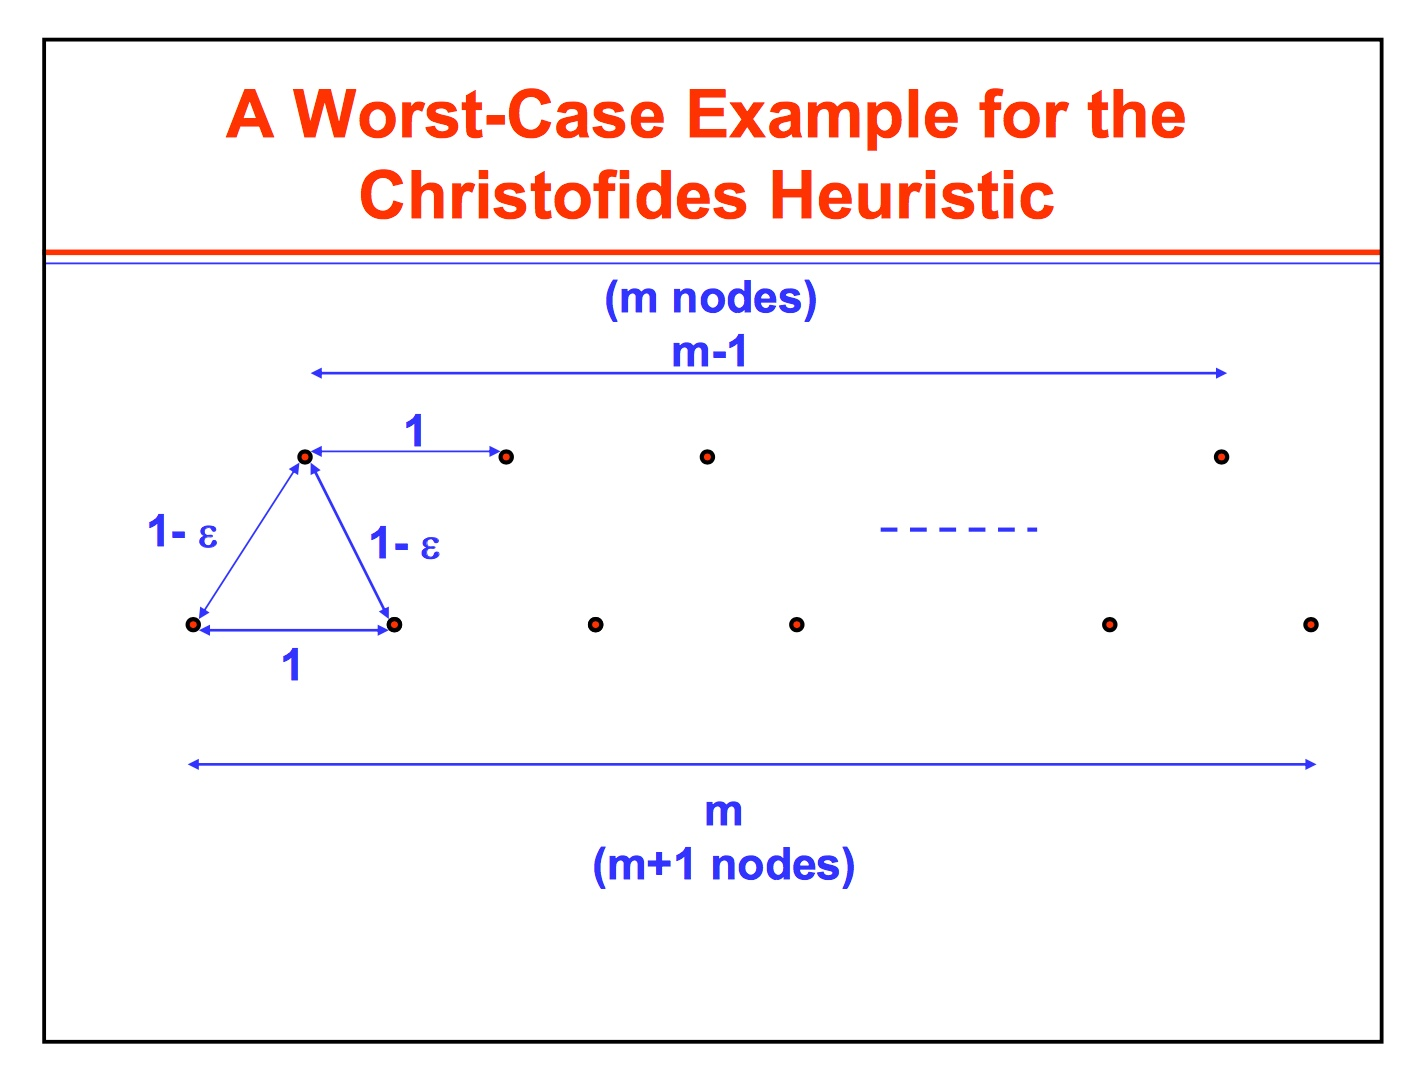
\includegraphics[scale=0.2]{worst1}
\end{center}
The MST of this graph will be a zig-zag path through the nodes, alternating between rows.  Only two nodes will have odd degree, the start and end of the path found by the MST (first and last node of the (m+1)-node row).  Christofides Algorithm will simply follow the path found in MST, and connect the first and last node. C$_c$ = 2m(d*)+m.\\
\begin{center}
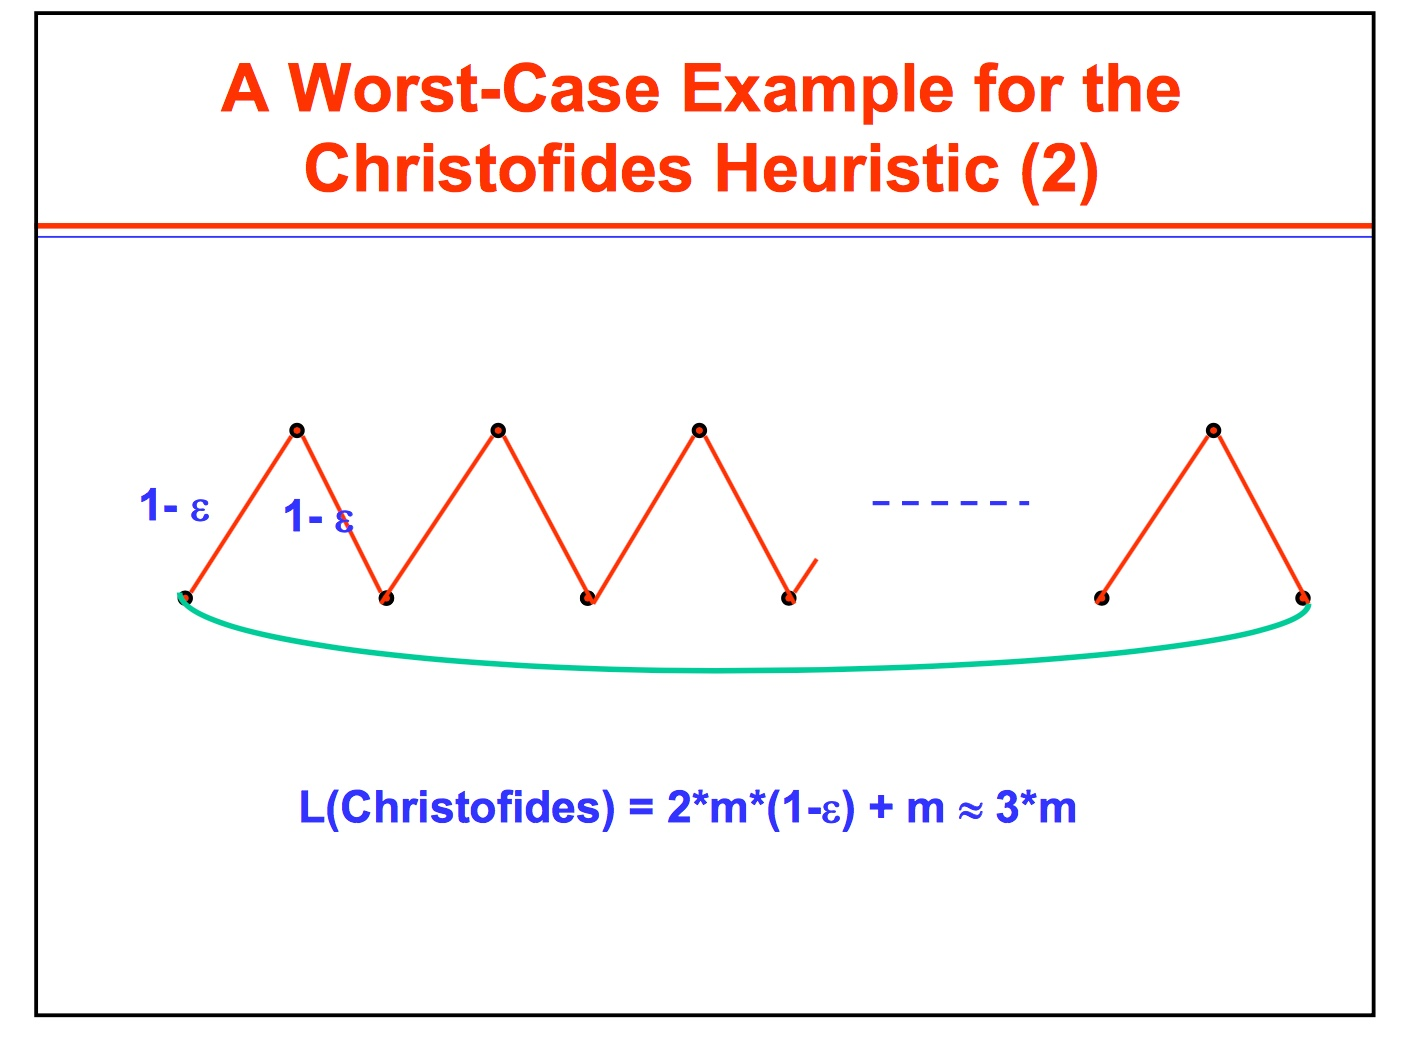
\includegraphics[scale=0.2]{worst2}
\end{center}
\indent The optimal solution in this case is to start at one end of either row, connect all nodes in the row linearly, connect to the nearest end of the next row, connect all nodes in that row linearly, and return to the starting node. C$_o$=m+m-1+2(d*)\\
\begin{center}
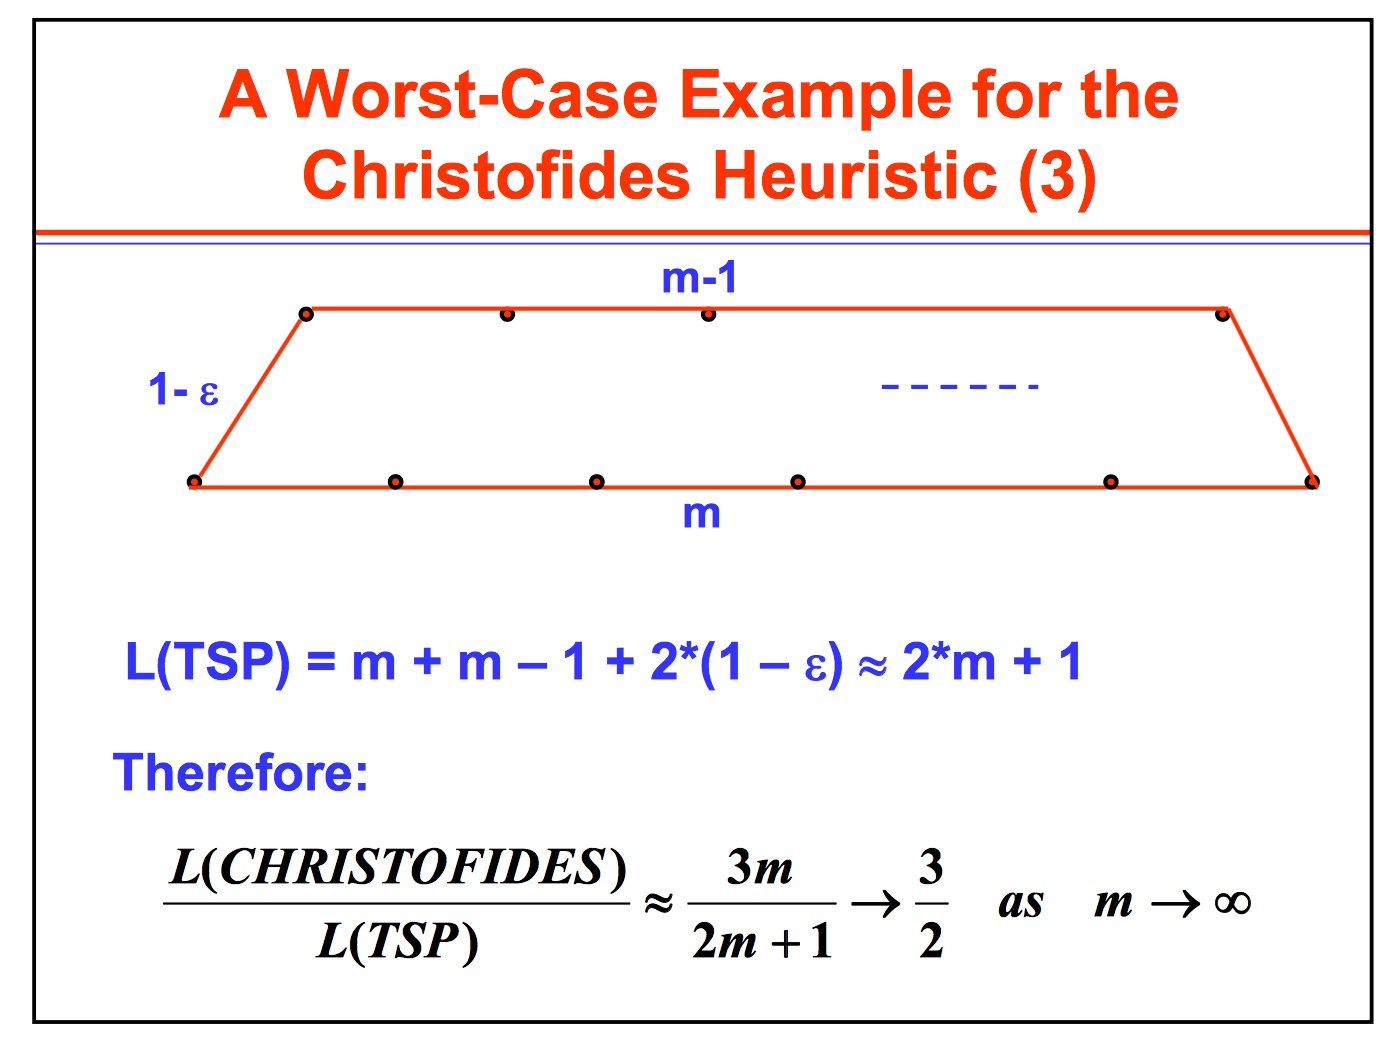
\includegraphics[scale=0.2]{worst3}
\end{center}
\indent In this case, the approximation ratio is $\frac{2m(d*)+m}{2m+2d*-1}$ =  $\frac{3m + 2d*}{2m + 2d* -1}$.  As $n \rightarrow \infty$, $\frac{3m + 2d*}{2m + 2d* -1}$ $\rightarrow$ $\frac{3}{2}$\\
* example and images from [7].\\
\subsubsection{Best-Case Input}
\indent\indent A best-case input for the Christofides Algorithm is one in which the optimal solution follows the edges of the MST on G to the fullest extent possible.  A trivial example of such a graph is a graph G with n nodes arranged linearly.  Distance between adjacent nodes d* =1.  Distance between first and last nodes = (n-1).  The MST of G will be a linear path through all nodes.  Every edge has length 1 for a total length n-1.  Christofides Algorithm will follow this MST through all nodes, then connect the two odd-degree nodes, first and last.  This will be identical to the optimal solution.\\
\begin{center}
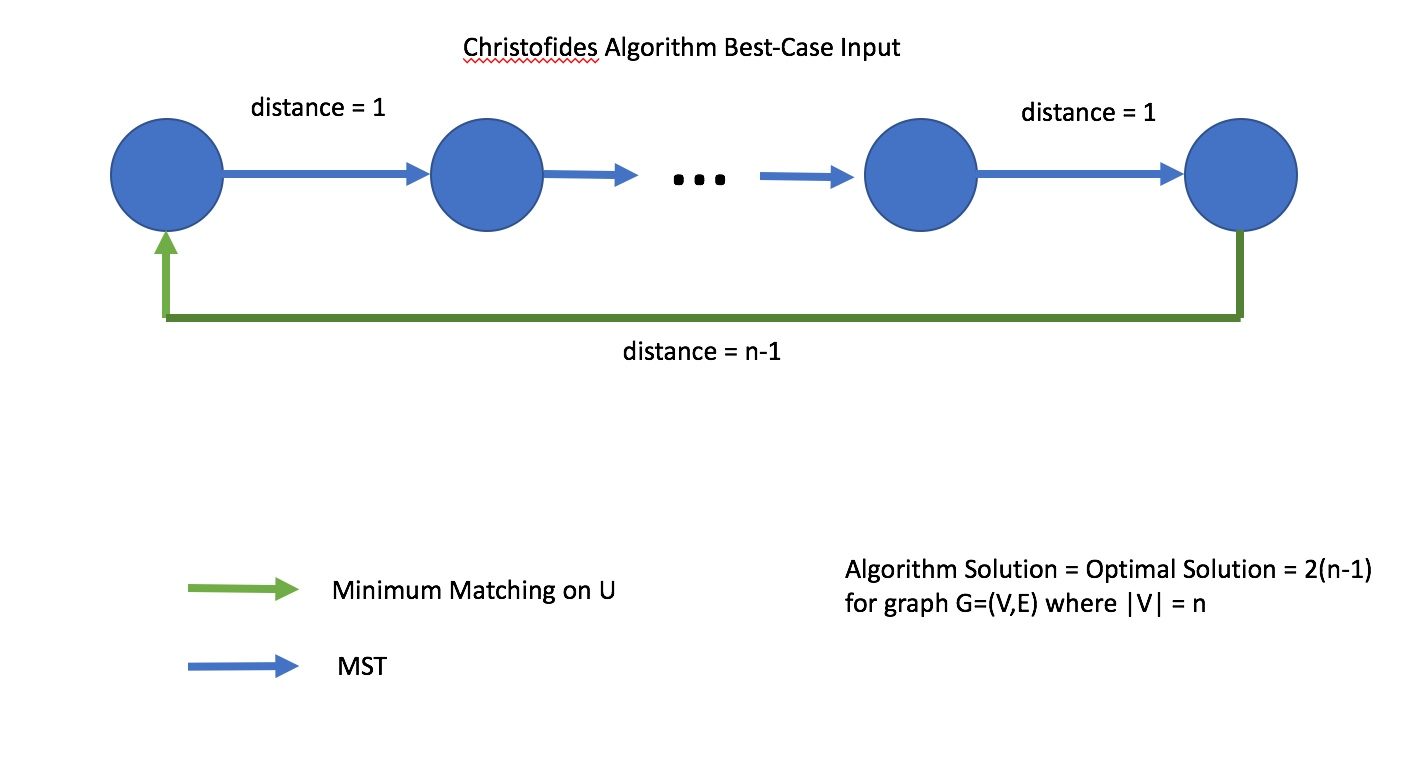
\includegraphics[scale=0.3]{best}
\end{center}
\subsubsection{Average-Case Input}
\indent\indent For most real-world graphs, the optimal solution will make use of some short-cuts that the algorithm will not, but not to the extent that we see in the worst-case scenario, above.  Results were obtained experimentally via random graph generation, and will be discussed in a following section.\\
\section{Experiment}
\subsection{Algorithm Implementation}
\indent\indent The Christofides Algorithm was implemented in Python, using networkX, numpy, and itertools libraries for implementation of helper functions.  Major steps of implementation were:\\
\indent 1.  Randomly generate graph.  Using a specified number of nodes \textit{n}, n random points were generated in a 1000 x 1000 unit 'space'.   Euclidean distances were then calculated between all nodes and stored in a numpy matrix for fast recall/operations.\\
\indent 2.  A graph object was generated using networkX functionality.  NetworkX was chosen for its useful graph functionality, such as finding MST and calculating maximum-weighted matchings.  This was easy to convert to a minimum-weight match.\\
\indent 3.  Using MST functionality of networkX, as described above, the MST of G was generated.\\
\indent 4.  Nodes of odd degree in MST were found.\\
\indent 5.  Minimum Matching was constructed via networkX Maximum Matching functionality.  To use networkX maximum matching functionality to make a minimum matching, I simply subtracted edge weights from an arbitrarily large number.  Smallest edge weights became largest, and vice-versa.  When constructing the graph based on this matching, I re-inserted the original edge weights.\\
\indent 6.  Merging was done via networkX add\_edges() method, and a Eulerian Circuit was generated via networkX eulerian\_circuit() method.\\
\indent 7.  Converting the Eulerian Circuit to Hamiltonian Circuit was trivial.  All that is required is to keep a list of visited nodes.  When a visited node is encountered a second time, simply continue along the Eulerian Circuit until a previously unvisited node is encountered.  Add nodes to a solution array in the order that they are visited.\\
\indent 8.  To calculate C$_c$, simply add up the edge costs to reflect the edges that are traversed, as reflected by the solution array.\\\\\\
\indent To compare algorithm results against optimal results, I simply brute-forced the same graphs that were randomly generated for the algorithm implementation.  Using itertools.permutations(), I generated all permutations of numbers of the set \{1,2,...,n-1\}.  0 was reserved as the start/finish node.  To avoid checking duplicate/reversed paths, any iteration where element[0] $<$ element[n] of the permutations was ignored.  Once permutations were generated and duplicates eliminated, distances were summed up to reflect the path generated by itertools. Time and path cost were recorded for all brute-force and algorithm iterations.\\
\subsection{Experiment Results}
\indent Data was collected over multiple iterations for n=[3,4,5,6,7,8,9,10,11,12,13].  Due to runtime constraints, number of iterations was decreased as n increased.  At n=3 to 10, 1000 iterations were performed.  At n=11 and 12, 100 iterations were performed, and at n=13, 50 iterations.  Beyond n=13, runtime was prohibitive.  Results are as follows:\\
\begin{center}
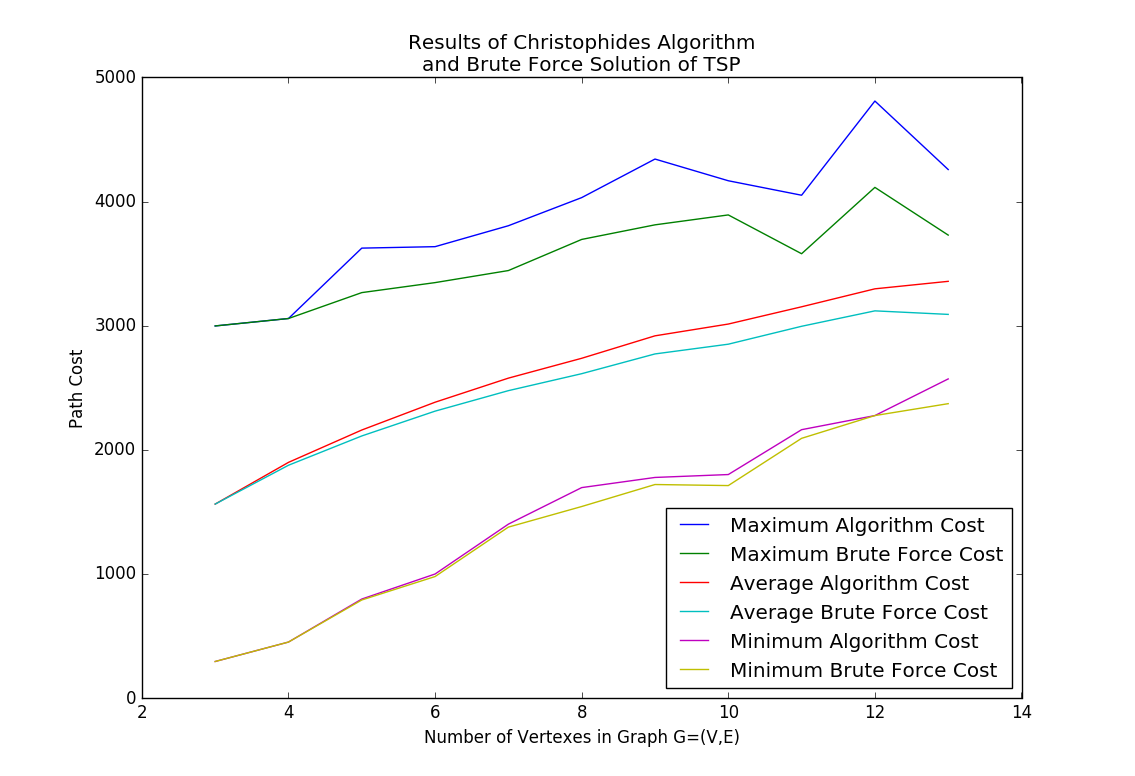
\includegraphics[scale=0.5]{cost}
\end{center}
\indent To measure accuracy of the Christofides Algorithm, we can compare average values of C$_c$ and C$_o$ for all n values for which simulations were run.\\
\begin{center}
\begin{tabular}{|c|c|c|}
\hline
C$_c$ & C$_o$ & $\frac{ALG}{OPT}$\\
\hline
1564.29889711  &  1564.29889711  &  1.0\\
\hline
1900.19945718  &  1877.04997719  &  1.0123329055\\
\hline
2160.71515929  &  2112.91559425  &  1.02262256248\\
\hline
2384.53768121  &  2312.67646758  &  1.03107274824\\
\hline
2578.42763296  &  2477.64256672  &  1.04067780704\\
\hline
2738.23113853  &  2614.22379746  &  1.04743562552\\
\hline
2919.01722133  &  2773.3136069  &  1.05253773467\\
\hline
3013.94297714  &  2851.72091876  &  1.05688567114\\
\hline
3152.81751083  &  2995.88517515  &  1.05238262701\\
\hline
3297.50312162  &  3120.09718795  &  1.05685910501\\
\hline
3357.8141498  &  3091.62924492  &  1.0860985855\\
\hline
\end{tabular}
\end{center}
\indent\indent From the above table, it appears that, on a graph of randomly-generated locations, Christofides Algorithm is well below the worst-case ratio of $\frac{3}{2}$.  However, there does appear to be a gradual increase in $\frac{OPT}{ALG}$ as \textit{n} increases.\\
\begin{center}
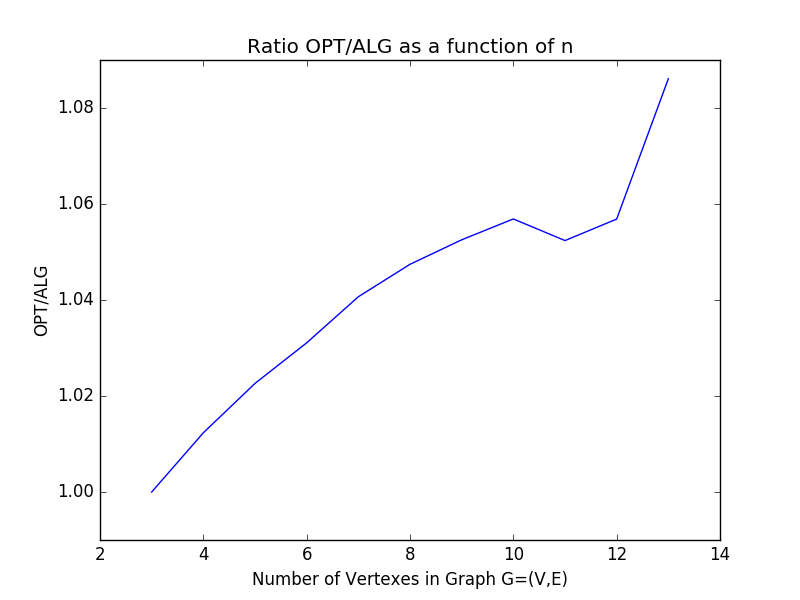
\includegraphics[scale=0.5]{costRatio.png}
\end{center}
\indent Similar examination of observed runtime of the algorithm and brute-force methods gives the following results:\\
\begin{center}
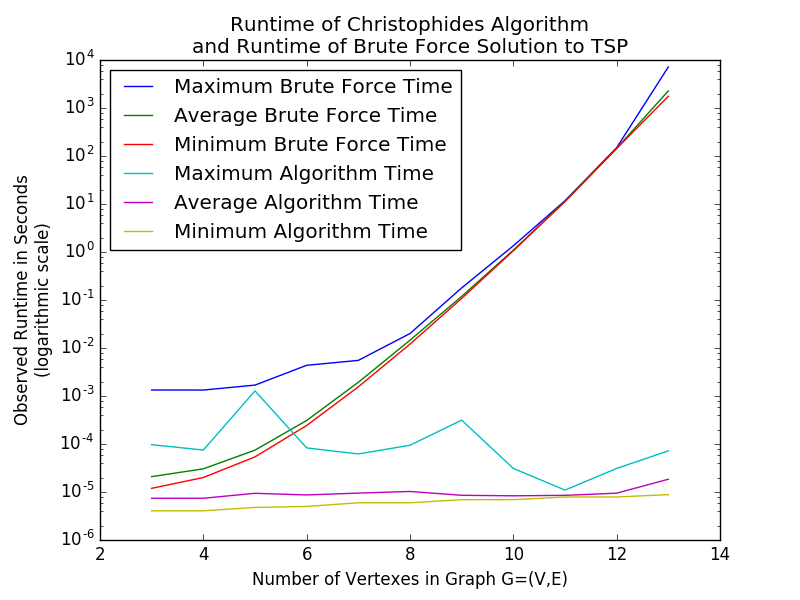
\includegraphics[scale=0.6]{time}
\end{center}
\indent\indent Observed runtime for the brute-force method increases rapidly as n increases.  Expected runtime of the brute-force method of solving the Travelling Salesman Problem was determined to be O((n-1)!), and the data of observed runtime seems to confirm that.  Observed runtime for the Christofides Algorithm appears to be mostly constant, with perhaps a very slight upward trend.  Expected runtime for Christofides Algorithm was determined to be O(n$^3$), but at such small values of n, it may be that runtime is being dominated by constant-time operations, such as overhead involved in function calls, etc.  As all coding was done in Python, with numpy used for matrix and numerical operations, this seems likely.  Operations implemented via numpy can be expected to complete much quicker than those implemented in pure Python, since numpy is implemented in C.\\
\indent To determine if the observed runtime matches expected, the ratio of $\frac{Brute-force\ Runtime}{Christofides\ Runtime}$ can be determined. Expected ratio is $\frac{(n-1)!}{n^3}$.\\
\begin{flushleft}
\begin{footnotesize}
\begin{tabular}{|c|c|c|c|c|c|}
\hline
n &{Brute-force Runtime} & Algorithm Runtime & $\frac{Brute-Force}{Algorithm}$ & $\frac{Expected\ brute\ force}{expected\ algorithm}$ & $\frac{observed\ ratio}{expected\ ratio}$\\
\hline
3&2.09114551544e-05  &  7.39550590515e-06  &  2.82758954189  &  0.222222222222  &  12.7241529385 \\
\hline
4&3.0389547348e-05  &  7.40838050842e-06  &  4.10205001126  &  0.375  &  10.93880003 \\
\hline
5&7.45985507965e-05  &  9.39774513245e-06  &  7.93792018672  &  0.96  &  8.26866686117 \\
\hline
6&0.000308976411819  &  8.68225097656e-06  &  35.5871320299  &  3.33333333333  &  10.676139609 \\
\hline
7&0.00192969703674  &  9.49168205261e-06  &  203.304011454  &  14.693877551  &  13.8359674462 \\
\hline
8&0.0145330505371  &  1.02622509003e-05  &  1416.16597356  &  78.75  &  17.9830599817 \\
\hline
9&0.118852747202  &  8.53967666626e-06  &  13917.7104528  &  497.777777778  &  27.9596861776 \\
\hline
10&1.0934151926  &  8.33058357239e-06  &  131253.132881  &  3628.8  &  36.1698448195 \\
\hline
11&11.388480289  &  8.51631164551e-06  &  1337254.99524  &  29990.0826446  &  44.5899069731 \\
\hline
12&144.883050308  &  9.45329666138e-06  &  15326193.1259  &  277200.0  &  55.2892969908 \\
\hline
13&2271.94656908  &  1.84488296509e-05  &  123148547.202  &  2834328.99408  &  43.4489247575 \\
\hline



\end{tabular}
\end{footnotesize}
\end{flushleft}
*numbers represent time in seconds for one iteration\\\\

\indent Since the observed ratio of $\frac{brute-force\ runtime}{algorithm\ runtime}$ is so much larger than the expected ratio, the observed ratio was divided by the expected ratio to see if there was a consistent relationship between the two, and that does, in fact, appear to be the case.  Trends in observed runtime appear to be in line with expected.\\
\section{Conclusions}
\indent\indent In this paper, we have examined the Christofides Algorithm in detail.  After examining the steps of the algorithm and proving the worst-case bound of $\frac{3}{2}$ of the optimal solution, experimental results were presented.  These results confirm the worst-case bound, and seem to indicate that average performance is closer to optimal than the worst case limit.  Observed runtime also appears to match expected runtime, O(n$^3$).  Comparison against a simple brute-force algorithm seems to confirm the expected runtime.
\newpage



\section{Sources}
\indent\indent  [1]	"Travelling salesman problem," in Wikipedia, Wikimedia Foundation, 2016. [Online]. Available: https://en.wikipedia.org/wiki/Travelling\_salesman\_problem. Accessed: Dec. 8, 2016.\\

[2] . Matai, S. Singh and M. Lal Mittal (2010). Traveling Salesman Problem: an Overview of Applications, Formulations, and Solution Approaches, Traveling Salesman Problem, Theory and Applications, Prof. Donald Davendra (Ed.), InTech, DOI: 10.5772/12909. Available from: http://www.intechopen.com/books/traveling-salesman-problem-theory-and-applications/traveling-salesman-problem-an-overview-of-applications-formulations-and-solution-approaches\\

[3]	T. H. Cormen, C. E. Leiserson, R. L. Rivest, and C. Stein, Introduction to Algorithms, 3rd ed. Cambridge, MA: The MIT Press, 2009.\\

[4] N. Christofides, Worst-case analysis of a new heuristic for the travelling salesman problem, Report 388, Graduate School of Industrial Administration, CMU, 1976.\\

[5] N. Christofides, The shortest hamiltonian chain of a graph, SIAMJ. on Appl. Math., 19, 1970, p. 689\\ 

[6]	C. H. Papadimitriou and K. Steiglitz, Combinatorial optimization: Algorithms and complexity. New York, NY, United States: Dover Publications, 2000.\\

[7]	[Online]. Available: https://ocw.mit.edu/courses/civil-and-environmental-engineering/1-203j-logistical-and-transportation-planning-methods-fall-2006/lecture-notes/lec15.pdf. Accessed: Dec. 9, 2016.
\end{document}  